% !TeX spellcheck = en_US
\documentclass[french]{yLectureNote}

\title{Électromagnétisme 3}
\subtitle{Physique}
\author{Paulhenry Saux}
\date{\today}
\yLanguage{Français}
%jesse.groenen@cemes.fr
\professor{M.Brut}
\usepackage{graphicx}%----pour mettre des images
\usepackage[utf8]{inputenc}%---encodage
\usepackage{geometry}%---pour modifier les tailles et mettre a4paper
%\usepackage{awesomebox}%---pour les boites d'exercices, de pbq et de croquis ---d\'esactiv\'e pour les TP de PC
\usepackage{tikz}%---pour deiffner + d\'ependance de chemfig
% \usepackage{tabularx}%---pour dimensionner automatiquement les tableaux avec variable X
\usepackage{awesomebox}%---Pour les boites info, danger et autres
\usepackage{menukeys}%---Pour deiffner les touches de Calculatrice
\usepackage{fancyhdr}%---pour les en-t\^ete personnalis\'ees
\usepackage{blindtext}%---pour les liens
\usepackage{hyperref}%---pour les liens (\`a mettre en dernier)
\usepackage{caption}%---pour la francisation de la l\'egende table vers Tableau
\usepackage{pifont}
\usepackage{array}%---pour les tableaux
\usepackage{lipsum}
\usepackage{yFlatTable}
\usepackage{multicol}
\usepackage{tabularx}
\usepackage{booktabs}
\newcommand{\Lim}[1]{\lim\limits_{\substack{#1}}\:}
\renewcommand{\vec}{\overrightarrow}
\newcommand{\N}[0]{\mathbb{N}}
\newcommand{\dd}{\mathrm{d}}
\newcommand{\norm}[1]{||\vec{#1}||}
\newcommand{\fo}{\psi(\vec{r},t)}
\newcommand{\foe}{\psi(\vec{r},t)\*}
\newcommand{\HH}{\hat{H}}
\newcommand{\hb}{\hbar}
\newcommand{\lap}{\nabla^2}
\newcommand{\lapcc}{\frac{\partial^2 }{\partial x^2}+\frac{\partial^2 }{\partial y^2}+\frac{\partial^2 }{\partial z^2}}
\newcommand{\E}{\vec{E}(M)}
\newcommand{\B}{\vec{B}(M)}
\newcommand{\V}{V(M)}
\newcommand{\er}{\vec{e_{\rho}}}
\newcommand{\ep}{\vec{e_{\varphi}}}
\newcommand{\pip}{\pi^+}
\newcommand{\pim}{\pi^-}
\newcommand{\mv}{\mathcal{V}}
\DeclareMathOperator{\Div}{Div}
\newcommand{\rot}{\vec{\mathrm{rot}}}
\newcommand{\grad}{\vec{\mathrm{grad}}}
%\setcounter{chapter}{3}
\begin{document}
%\chapter{Puissance et énergie du champ Em}
\setcounter{chapter}{3}
\chapter{Polarisation : aspects microscopiques}
\criticalInfo{Rappel}{n conducteur parfait est équivalent à un milieu infiniment polarisable : $\chi_e \to \infty$. L'écrantage est total : $\vec{E_{int}} = \vec{0}$.
 C'est équivalent en polarisation alors qu'il n'y a pas de dipôle élémentaire. C'est un réservoir illimité d'électrons libres.
}

\section{Polarisabilité}
\subsection{Définition}[Polarisabilité]
On se place en échelle microscopique
\begin{definition}
    $$\vec{p_j} = \epsilon_0 \alpha_j \vec{e_{loc}(M_j)}$$ avec $\vec{p_j}$ le moment dipolaire électrique induit sur l'élément j , $\vec{e_{loc}}$ le champ électrique micorcopique perçu au site $j$ par le constituant élémentaire
    et $\alpha_j$ la Polarisabilité de l'élément j.
\end{definition}
\warningInfo{Champ local}{
    $\vec{e_{loc}}$ correspond au champ appliqué $\vec{E_a}$ + champ microscopique crée par les constituants du milieu entourant $M_j$.

    $\alpha_j$ est une constante positive.
}
\subsection{Bilan}
\begin{itemize}
    \item Polarisation électronique : Modification de la répartiiton des charges internes à haque atome ou ion, toujours présente
    \item Polarisation atomique : Déplacement des atomes/ions par rapport à leur posiuton d'équilibre
    \item Polarisation d'orienrttaion : Orientation du moment dipolaire permananr d'une molcéule polaire. Nécessite une liberté de mouvement. Cela concerne donc les fluides.
\end{itemize}
\subsection{Modélisation}
\subsubsection{Polarisabilité électronique}
\begin{theorem}[Polarisabilité $\alpha_e$ selon Mossoti]
    $\alpha_e = 4\pi a^3 = \frac{Z^2z^2}{\epsilon_0m_e\omega_0^2}$ avec $\omega_0^2 = \frac{K}{m_e}$
\end{theorem}
\subsubsection{Polarisabilié atomique et ionique}
\begin{theorem}
    $$\alpha_a = \alpha_i = \frac{q^2}{\epsilon_0\mu \omega_0^2}$$
\end{theorem}

\section{Champ local - champ macroscopique}
On rappelle que généralement, $\vec{e_{loc}}\neq \vec{E}$
\subsection{Gaz et milieux dilués}
Dans le cas d'un gaz sous faible pression, on néglige l'intéraction entre dipole sous l'échelle microscopique, on a donc 
$\vec{e_{loc}}\simeq \vec{E}$ pour les milieux dilués.

\section{Lien entre polarisabilité et permitivité diélectrique}
\subsection{Gaz dilués}
\begin{theorem}[Relation de Langevin Debye]
    $$(\epsilon_r-1)\frac{M}{\rho^*}=N_A\alpha$$ avec $\rho^*$ la masse volumique et $\alpha = \alpha_e+\alpha_a+\alpha_{or}$
\end{theorem}

\section{Aspects dynamiques}
On considère un milieu soumis à un champ électrique sinusoidal de pulsation $\omega$.
\subsection{Modèle de Drude-Lorenz}
\begin{theorem}[Modèle de Drude]
    $$m_e\frac{\dd^2 \vec{r}}{\dd t^2}=-K\vec{r}-\frac{m_e}{\tau}\frac{\dd \vec{r}}{\dd t}-e(\vec{E}+\frac{\dd \vec{r}}{\dd t}\wedge \vec{B})$$
\end{theorem}
\subsection{Susceptibilité et permittivité complexe}
On repasse en macro.
\begin{itemize}
    \item $\omega_0$ est la pulsation propre
    \item $\omega_p^2 = \frac{n_ve^2}{m_e\epsilon_0}$ la force d'oscillateur
    \item $\tau$ caractérise l'amortissement. Si $\tau >> 1$, pas d'amortissement
    \item La partie imaginaire est toujours positive
\end{itemize}
\subsection{Lien entre absorption des ondes et Partie imaginaire de er}
On se place à $\omega = \omega_0$

on utilise les valeurs réelles et non les valeurs complexes\marginInfo{En effet, on effectu un produit et le produit des parties réelles n'est pas la partie réelle du produit}
\begin{theorem}
    $$<P_m>_T = \frac{V}{2}\omega_0 \epsilon_0 (Im(e_r))E_0^2$$
\end{theorem}
On remarque que s'il il n'y a pas de frottement, il n'y a pas d'absorption.
\section{Bilan}
les différents mécanismes s'ajoutent mais ont des pulsation différentes.
\begin{itemize}
    \item Polarisabilité : toujours présente = Gamme UV
    \item Polarisabilité ionique et atomique  : dépend de la polarité de la liaison ($\varnothing$ si liaison covalente) = IR lointain
    \item Polarisabiluté d'orientation : mécanisme différente, pas de résonance les collisions dominent. = Gamme micro-ondes
\end{itemize}
En notant $$\underline{\chi}=\underline{\chi_{or}}+\underline{\chi_i}+\underline{\chi_e}$$ 

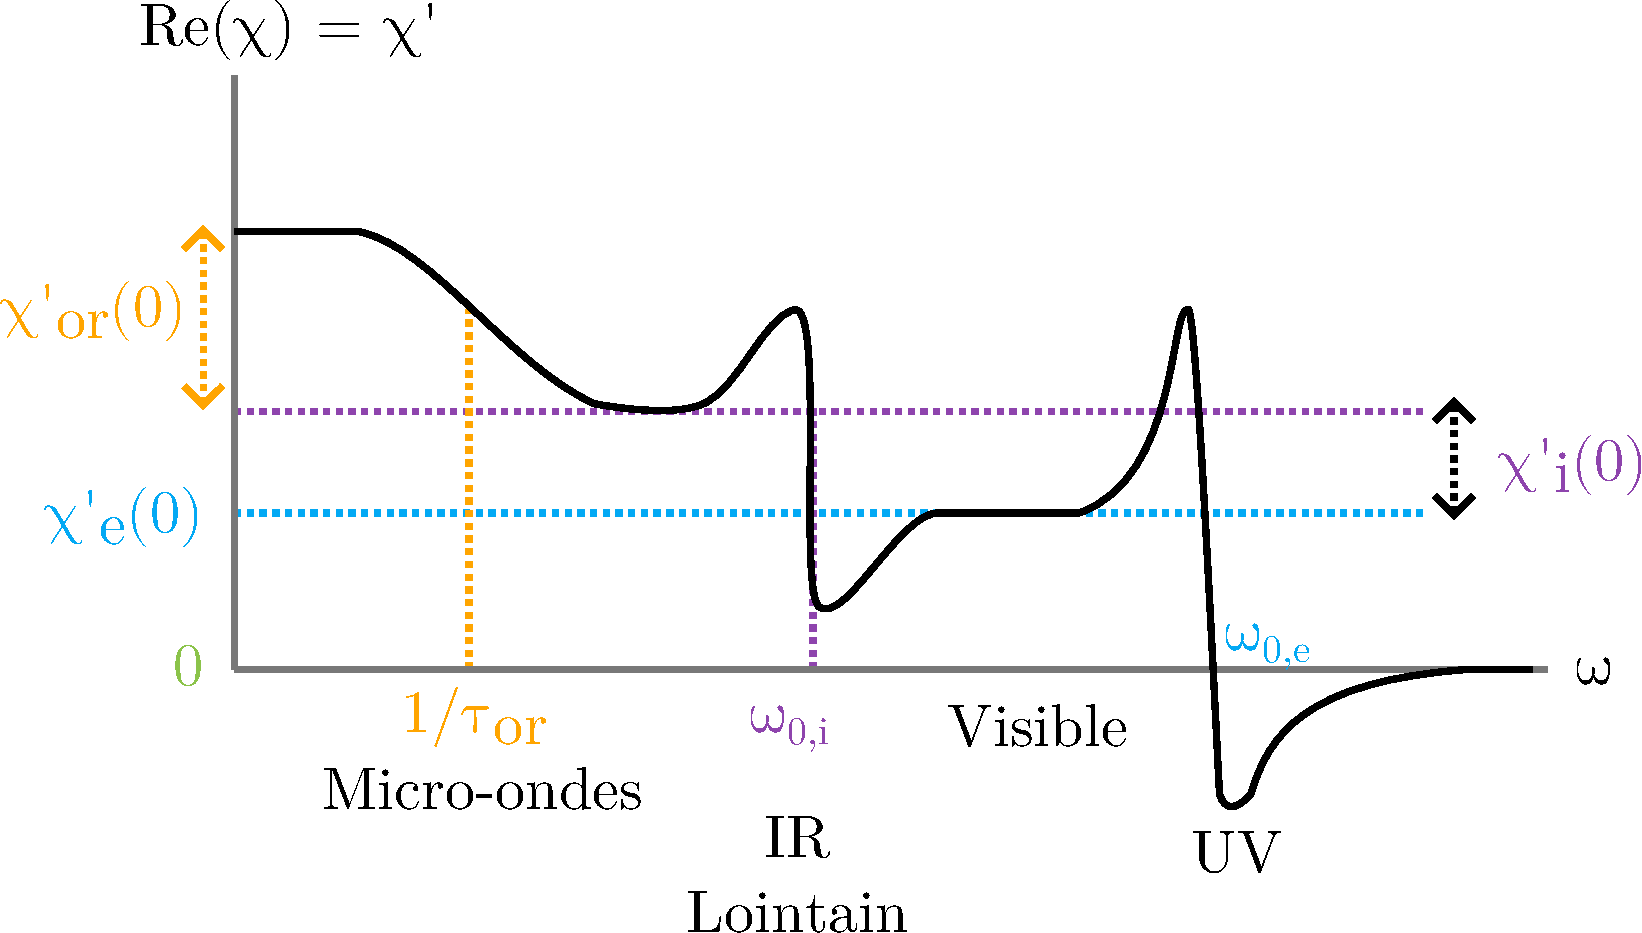
\includegraphics[scale=0.5]{schema_bilan.pdf}
\end{document}
